%%%%%%%%%%%%%%%%%%%%%%%%%%%%%%%%%%%%%%%%%%%%%%%%%%%%%%%%%%%%%%%%%%%%%%%%%%%%%%%%%%%%%%%%%%%%%%%%%%%%%%%%%%%%%%%%%%%%%%%%%%%%%%%%%%%%%%%%%%%%%%%%%

\UC{Aggiunta prodotto al carrello dalla PDP}
\label{aggiunta-carrello-pdp}

\begin{figure}[H]
	\centering
	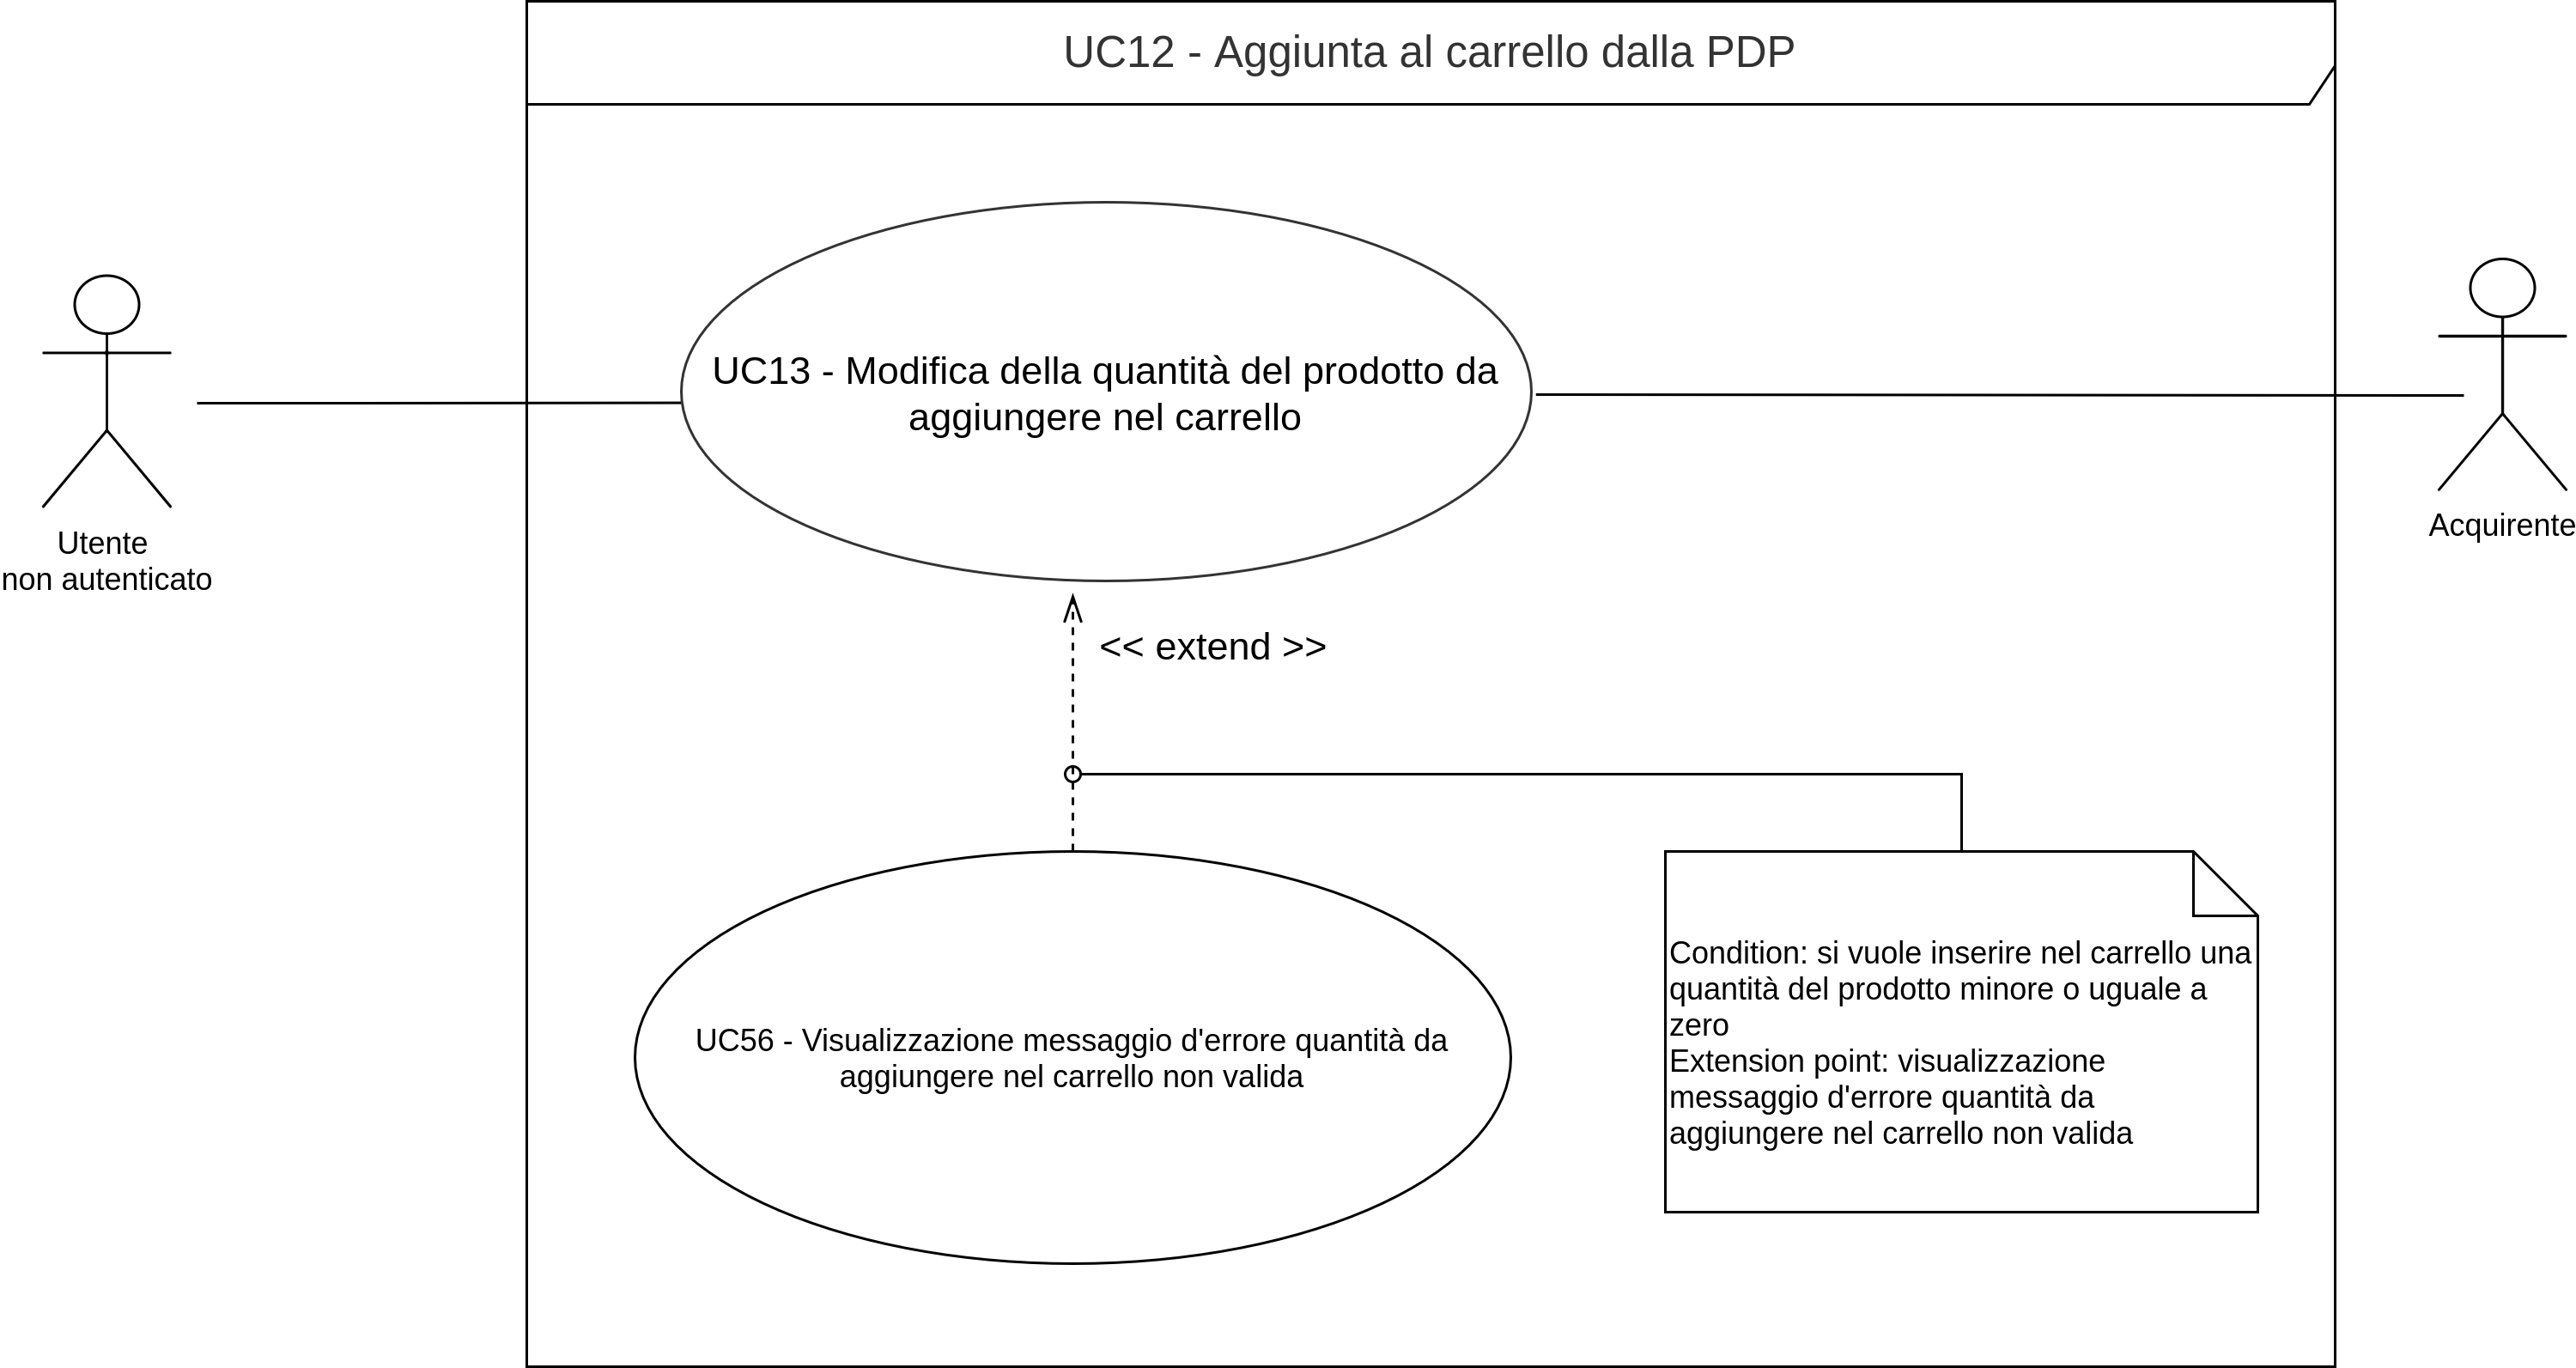
\includegraphics[scale=0.4]{Immagini/DiagrammiUC/Acquirente/AggiuntaProdottiCarrelloPDP.png}
	\caption{Diagramma di \actualUC: Aggiunta al carrello dalla PDP}
	\label{fig:aggiunta-carrello-pdp}
\end{figure}

L'acquirente o l'utente non autenticato si trova nella \glo{PDP} del prodotto che vuole aggiungere al suo carrello.
\begin{itemize}
    \item \textbf{Attori primari:} acquirente o utente non autenticato;
    \item \textbf{Precondizione:} l'attore si trova nella PDP del prodotto;
    \item \textbf{Postcondizione:} il prodotto è stato aggiunto al carrello dell'attore;
    \item \textbf{Scenario principale:} l'attore vuole comprare il prodotto visualizzato dalla PDP e in tal caso:
    \begin{itemize}
        \item (UC\ref{modifica-quantita-da-aggiungere-al-carrello}) - Modifica la quantità del prodotto da aggiungere nel carrello;
        \item Seleziona la funzione di aggiunta al carrello del seguente prodotto nella quantità impostata.
    \end{itemize}
\end{itemize}

%%%%%%%%%%%%%%%%%%%%%%%%%%%%%%%%%%%%%%%%%%%%%%%%%%%%%%%%%%%%%%%%%%%%%%%%%%%%%%%%%%%%%%%%%%%%%%%%%%%%%%%%%%%%%%%%%%%%%%%%%%%%%%%%%%%%%%%%%%%%%%%%% 

\UC{Modifica della quantità del prodotto da aggiungere nel carrello}
\label{modifica-quantita-da-aggiungere-al-carrello}

L'acquirente o l'utente non autenticato modifica la quantità del prodotto che vuole aggiungere nel carrello.
\begin{itemize}
	\item \textbf{Attori primari:} acquirente o utente non autenticato;
	\item \textbf{Precondizione:} l'attore vuole aggiungere un prodotto nel carrello e desidera modificarne la quantità da aggiungere;
	\item \textbf{Postcondizione:} la quantità del prodotto da aggiungere nel carrello è aggiornata;
	\item \textbf{Scenario principale:} l'attore vuole aggiungere un prodotto nel carrello e desidera modificarne la quantità da aggiungere. Per farlo dovrà selezionare la funzione per aumentare o diminuire la quantità del prodotto.
	\item \textbf{Scenari alternativi:}
	\begin{enumerate}[label=\lett]
        \item Se non viene modificata la quantità del prodotto da aggiungere nel carrello, allora verrà aggiunta un'unità di quel prodotto.
    \end{enumerate}
	\item \textbf{Estensioni:}
	\begin{enumerate}[label=\lett]
        \item L'attore inserire una quantità minore o uguale a zero. Per questo motivo:
        \begin{itemize}
            \item (UC\ref{estensione:quantita-da-aggiungere-al-carrello-non-valida}) - Viene visualizzato il messaggio d'errore quantità da aggiungere al carrello non valida;
            \item Verrà impedita l'aggiunta al carrello.
        \end{itemize}
	\end{enumerate}
\end{itemize}

%%%%%%%%%%%%%%%%%%%%%%%%%%%%%%%%%%%%%%%%%%%%%%%%%%%%%%%%%%%%%%%%%%%%%%%%%%%%%%%%%%%%%%%%%%%%%%%%%%%%%%%%%%%%%%%%%%%%%%%%%%%%%%%%%%%%%%%%%%%%%%%%% 
